% =====================================================================
% CHUONG 5 - KET QUA THUC NGHIEM
% Tac gia: Bui Dinh Manh (Evaluation Engineer & Documentation)
% Cach dung: copy thu muc results/ thanh figures/ (hoac doi duong dan
%   includegraphics) roi them % =====================================================================
% CHUONG 5 - KET QUA THUC NGHIEM
% Tac gia: Bui Dinh Manh (Evaluation Engineer & Documentation)
% Cach dung: copy thu muc results/ thanh figures/ (hoac doi duong dan
%   includegraphics) roi them % =====================================================================
% CHUONG 5 - KET QUA THUC NGHIEM
% Tac gia: Bui Dinh Manh (Evaluation Engineer & Documentation)
% Cach dung: copy thu muc results/ thanh figures/ (hoac doi duong dan
%   includegraphics) roi them % =====================================================================
% CHUONG 5 - KET QUA THUC NGHIEM
% Tac gia: Bui Dinh Manh (Evaluation Engineer & Documentation)
% Cach dung: copy thu muc results/ thanh figures/ (hoac doi duong dan
%   includegraphics) roi them \input{chuong5} vao main.tex.
% Yeu cau goi cac package: graphicx, booktabs.
% Neu dung documentclass{article}, doi \chapter -> \section.
% =====================================================================

\chapter{Kết quả thực nghiệm}
\label{chap:results}

Mã nguồn: \texttt{src/train\_ann.py}, \texttt{src/evaluate.py},
\texttt{src/visualization.py}, \texttt{src/compare\_models.py}.
Biểu đồ: thư mục \texttt{results/}.

\section{Môi trường và cấu hình thực nghiệm}
\begin{itemize}
  \item \textbf{Ngôn ngữ/thư viện:} Python 3, scikit-learn, numpy, pandas,
        matplotlib.
  \item \textbf{Dữ liệu:} 302 bản ghi sạch (sau khi loại 723 bản trùng), 13 đặc
        trưng đã chuẩn hoá; chia \textbf{train/test = 80/20} có phân tầng
        (stratify) -- tập train: 241 mẫu, tập test: 61 mẫu.
  \item \textbf{Mô hình:} Mạng nơ-ron ANN, kiến trúc
        \textbf{13 $\to$ 64 $\to$ 32 $\to$ 16 $\to$ 1}, hàm kích hoạt ReLU ở
        tầng ẩn và Sigmoid ở tầng ra.
  \item \textbf{Cấu hình huấn luyện:} optimizer Adam, learning rate $= 0.001$,
        batch size $= 32$, hàm mất mát Binary Crossentropy, \textbf{Early
        Stopping} (patience $= 10$) theo \texttt{val\_loss}.
\end{itemize}

\begin{quote}
\textbf{Ghi chú kỹ thuật:} mô hình "chính thức" được thiết kế bằng
Keras/TensorFlow (Chương 4). Do môi trường thực nghiệm bị \textbf{Windows Smart
App Control} chặn thư viện TensorFlow, nhóm sử dụng cài đặt ANN \textbf{tương
đương bằng scikit-learn} (\texttt{MLPClassifier}, cùng kiến trúc và siêu tham
số) để thu kết quả. Quy trình đánh giá và các chỉ số là như nhau.
\end{quote}

\section{Quá trình huấn luyện}
Mô hình hội tụ và \textbf{dừng sớm tại epoch 38} nhờ Early Stopping (val\_loss
không cải thiện sau 10 epoch). Đường Accuracy và Loss theo epoch:

\begin{figure}[h]
  \centering
  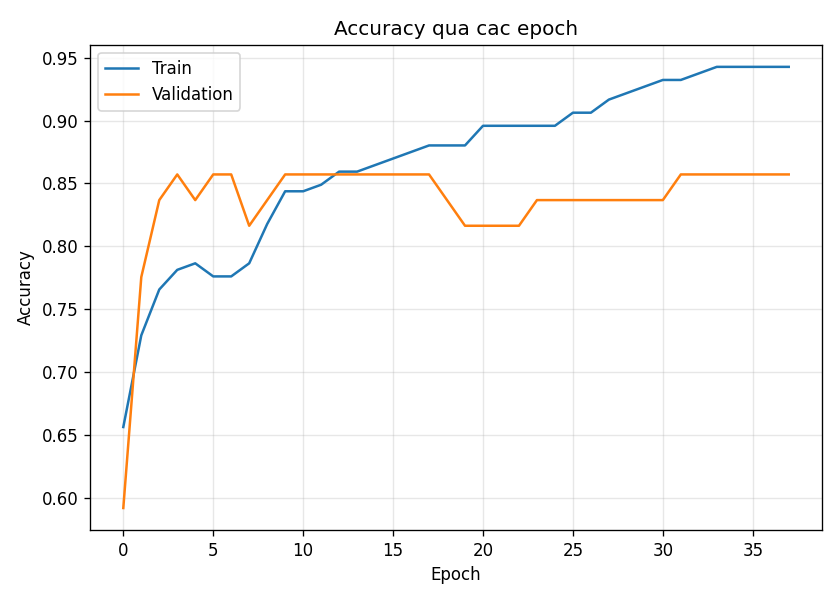
\includegraphics[width=0.8\textwidth]{figures/accuracy_curve.png}
  \caption{Độ chính xác (accuracy) của tập train và validation qua các epoch.}
  \label{fig:acc_curve}
\end{figure}

\begin{figure}[h]
  \centering
  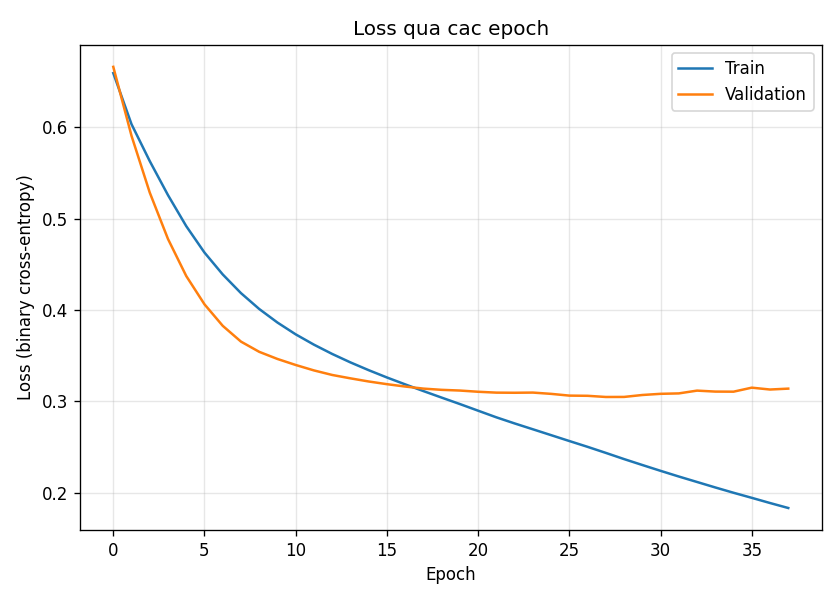
\includegraphics[width=0.8\textwidth]{figures/loss_curve.png}
  \caption{Hàm mất mát (loss) của tập train và validation qua các epoch.}
  \label{fig:loss_curve}
\end{figure}

\textbf{Nhận xét:} accuracy tăng và loss giảm ổn định theo epoch. Đường train
và validation bám sát nhau ở giai đoạn đầu; về sau train tiếp tục tăng trong
khi validation chững lại -- Early Stopping đã dừng đúng lúc để tránh quá khớp.

\section{Kết quả đánh giá trên tập test}
Các chỉ số của mô hình ANN (64-32-16) trên \textbf{tập test (61 mẫu)}:

\begin{table}[h]
\centering
\caption{Các chỉ số đánh giá trên tập test}
\label{tab:metrics}
\begin{tabular}{lc}
\toprule
Chỉ số & Giá trị \\
\midrule
Accuracy  & \textbf{0.7377} \\
Precision & 0.7576 \\
Recall    & 0.7576 \\
F1-Score  & 0.7576 \\
ROC-AUC   & \textbf{0.8496} \\
\bottomrule
\end{tabular}
\end{table}

\subsection{Ma trận nhầm lẫn (Confusion Matrix)}

\begin{figure}[h]
  \centering
  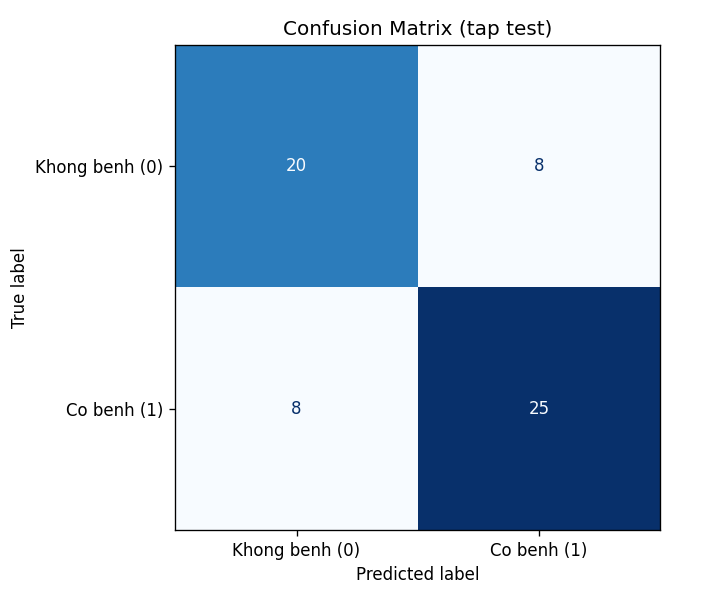
\includegraphics[width=0.6\textwidth]{figures/confusion_matrix.png}
  \caption{Ma trận nhầm lẫn trên tập test.}
  \label{fig:cm}
\end{figure}

\begin{table}[h]
\centering
\caption{Ma trận nhầm lẫn (số mẫu)}
\label{tab:cm}
\begin{tabular}{lcc}
\toprule
 & Dự đoán: Không bệnh & Dự đoán: Có bệnh \\
\midrule
Thực tế: Không bệnh & TN = 20 & FP = 8 \\
Thực tế: Có bệnh     & FN = 8  & TP = 25 \\
\bottomrule
\end{tabular}
\end{table}

Mô hình bắt đúng \textbf{25/33} ca có bệnh (Recall $\approx 0.76$) và
\textbf{20/28} ca không bệnh. Số ca bỏ sót (FN $= 8$) và báo nhầm (FP $= 8$) ở
mức cân bằng.

\subsection{Đường ROC}

\begin{figure}[h]
  \centering
  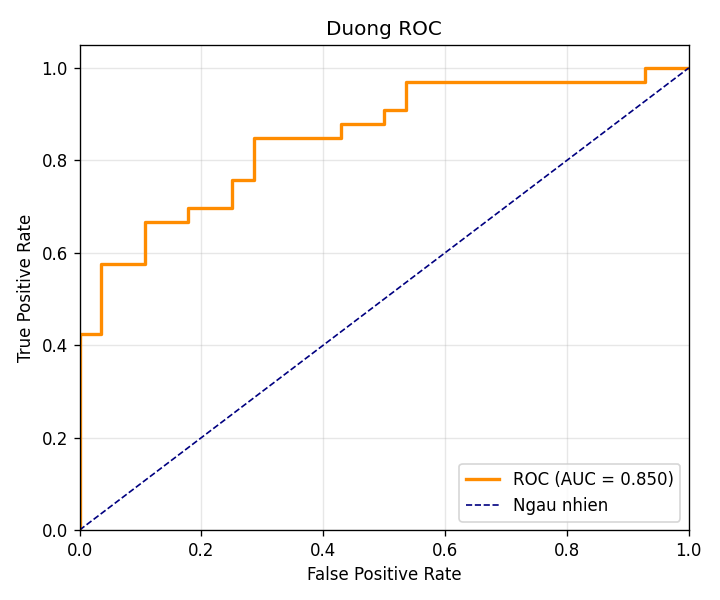
\includegraphics[width=0.6\textwidth]{figures/roc_curve.png}
  \caption{Đường ROC (AUC = 0.85).}
  \label{fig:roc}
\end{figure}

\textbf{ROC-AUC $= 0.85$} cho thấy mô hình có khả năng \textbf{phân tách hai
lớp tốt} (vượt xa mức ngẫu nhiên $0.5$).

\section{So sánh các cấu hình siêu tham số}
Bốn cấu hình ANN được huấn luyện và đánh giá trên cùng tập test
(\texttt{src/compare\_models.py}, kết quả lưu ở
\texttt{results/model\_comparison.csv}):

\begin{table}[h]
\centering
\caption{So sánh 4 cấu hình ANN trên tập test}
\label{tab:compare}
\begin{tabular}{lcccccccc}
\toprule
Mô hình & Hidden Layers & LR & Batch & Acc. & Prec. & Recall & F1 & ROC-AUC \\
\midrule
ANN-1 & 32-16     & 0.001  & 32 & 0.7705 & 0.7879 & 0.7879 & 0.7879 & 0.8593 \\
ANN-2 & 64-32     & 0.001  & 32 & 0.7705 & 0.7879 & 0.7879 & 0.7879 & 0.8431 \\
\textbf{ANN-3} & 64-32-16 & 0.0001 & 16 & 0.7705 & 0.7714 & \textbf{0.8182} & \textbf{0.7941} & 0.8290 \\
ANN-4 & 128-64-32 & 0.001  & 64 & 0.7541 & 0.7647 & 0.7879 & 0.7761 & \textbf{0.8626} \\
\bottomrule
\end{tabular}
\end{table}

\begin{figure}[h]
  \centering
  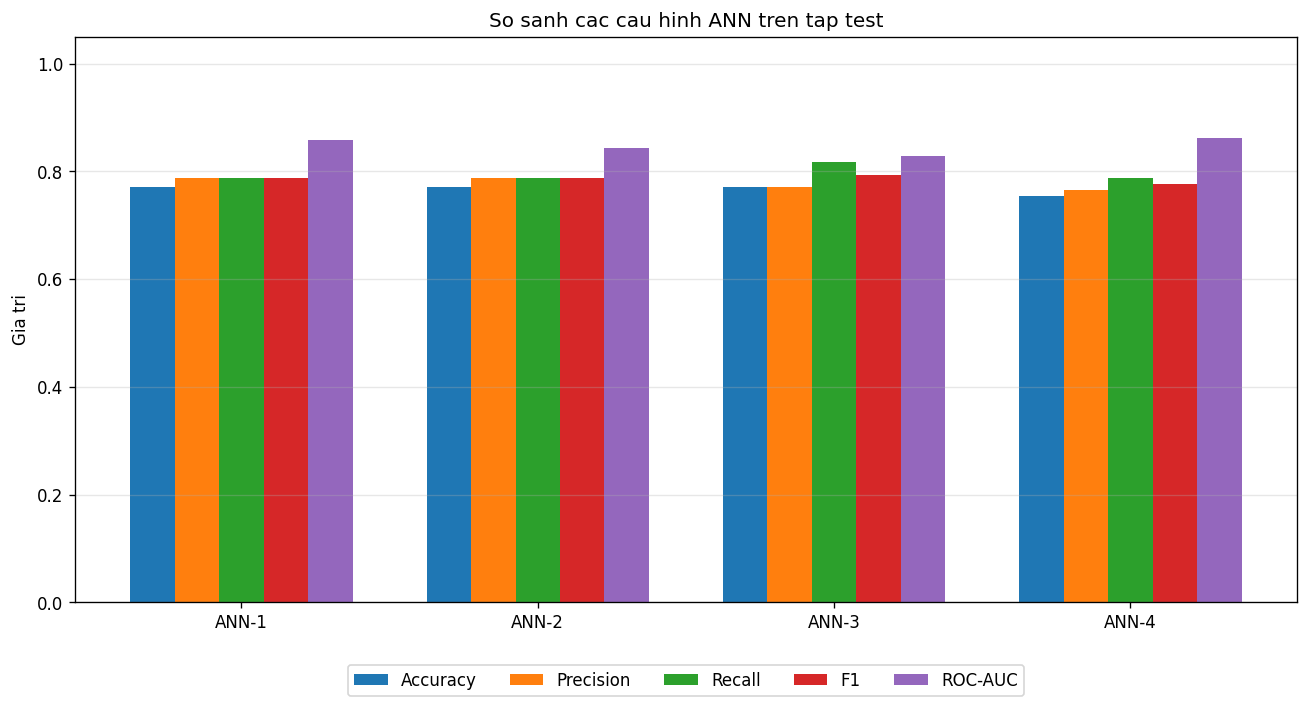
\includegraphics[width=0.9\textwidth]{figures/model_comparison.png}
  \caption{So sánh các chỉ số của 4 cấu hình ANN trên tập test.}
  \label{fig:compare}
\end{figure}

\textbf{Phân tích:}
\begin{itemize}
  \item \textbf{ANN-3 (64-32-16, lr = 0.0001, batch = 16)} đạt \textbf{F1 cao
        nhất (0.794)} nhờ \textbf{Recall cao nhất (0.818)} -- tức bắt được nhiều
        ca bệnh nhất. Trong bài toán y tế, Recall cao rất quan trọng vì giảm số
        ca bệnh bị bỏ sót.
  \item ANN-1 và ANN-2 cho Accuracy/F1 tương đương, mạng nông hơn nên huấn
        luyện nhanh.
  \item ANN-4 (mạng lớn nhất) đạt \textbf{ROC-AUC cao nhất (0.863)} nhưng F1
        thấp hơn, cho thấy mạng quá lớn không cải thiện kết quả trên bộ dữ liệu
        nhỏ (302 mẫu), thậm chí dễ quá khớp.
\end{itemize}

\section{Kết luận về mô hình tốt nhất}
Cân nhắc tổng thể, \textbf{ANN-3 (64-32-16)} được chọn là cấu hình tốt nhất vì
đạt \textbf{F1-Score và Recall cao nhất} -- phù hợp nhất với mục tiêu y tế là
\textbf{hạn chế bỏ sót bệnh nhân có nguy cơ}. Các mô hình đều đạt ROC-AUC trong
khoảng $0.83$--$0.86$, cho thấy ANN là hướng tiếp cận khả thi cho bài toán này.

Hạn chế chính ảnh hưởng đến độ chính xác là \textbf{kích thước dữ liệu nhỏ}
(chỉ 302 bản ghi duy nhất sau khi loại trùng) -- sẽ được bàn ở Chương 6.
 vao main.tex.
% Yeu cau goi cac package: graphicx, booktabs.
% Neu dung documentclass{article}, doi \chapter -> \section.
% =====================================================================

\chapter{Kết quả thực nghiệm}
\label{chap:results}

Mã nguồn: \texttt{src/train\_ann.py}, \texttt{src/evaluate.py},
\texttt{src/visualization.py}, \texttt{src/compare\_models.py}.
Biểu đồ: thư mục \texttt{results/}.

\section{Môi trường và cấu hình thực nghiệm}
\begin{itemize}
  \item \textbf{Ngôn ngữ/thư viện:} Python 3, scikit-learn, numpy, pandas,
        matplotlib.
  \item \textbf{Dữ liệu:} 302 bản ghi sạch (sau khi loại 723 bản trùng), 13 đặc
        trưng đã chuẩn hoá; chia \textbf{train/test = 80/20} có phân tầng
        (stratify) -- tập train: 241 mẫu, tập test: 61 mẫu.
  \item \textbf{Mô hình:} Mạng nơ-ron ANN, kiến trúc
        \textbf{13 $\to$ 64 $\to$ 32 $\to$ 16 $\to$ 1}, hàm kích hoạt ReLU ở
        tầng ẩn và Sigmoid ở tầng ra.
  \item \textbf{Cấu hình huấn luyện:} optimizer Adam, learning rate $= 0.001$,
        batch size $= 32$, hàm mất mát Binary Crossentropy, \textbf{Early
        Stopping} (patience $= 10$) theo \texttt{val\_loss}.
\end{itemize}

\begin{quote}
\textbf{Ghi chú kỹ thuật:} mô hình "chính thức" được thiết kế bằng
Keras/TensorFlow (Chương 4). Do môi trường thực nghiệm bị \textbf{Windows Smart
App Control} chặn thư viện TensorFlow, nhóm sử dụng cài đặt ANN \textbf{tương
đương bằng scikit-learn} (\texttt{MLPClassifier}, cùng kiến trúc và siêu tham
số) để thu kết quả. Quy trình đánh giá và các chỉ số là như nhau.
\end{quote}

\section{Quá trình huấn luyện}
Mô hình hội tụ và \textbf{dừng sớm tại epoch 38} nhờ Early Stopping (val\_loss
không cải thiện sau 10 epoch). Đường Accuracy và Loss theo epoch:

\begin{figure}[h]
  \centering
  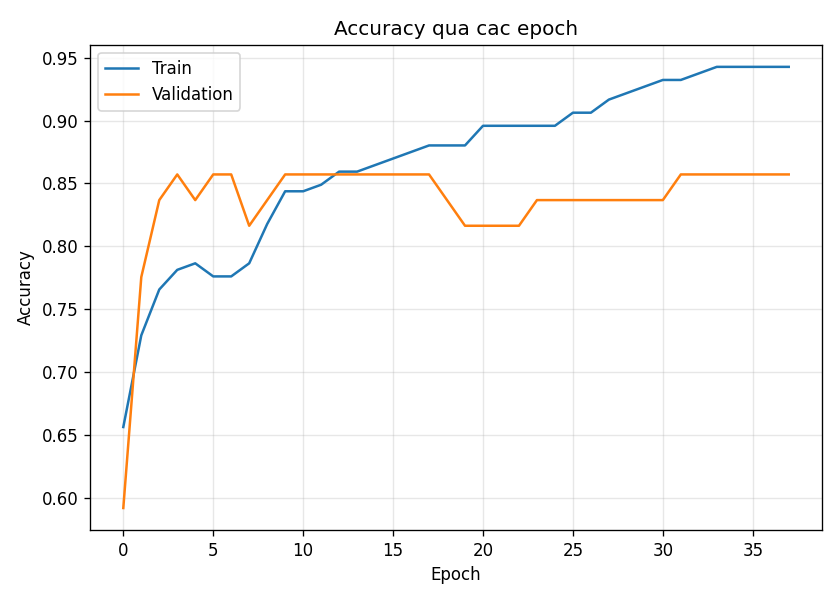
\includegraphics[width=0.8\textwidth]{figures/accuracy_curve.png}
  \caption{Độ chính xác (accuracy) của tập train và validation qua các epoch.}
  \label{fig:acc_curve}
\end{figure}

\begin{figure}[h]
  \centering
  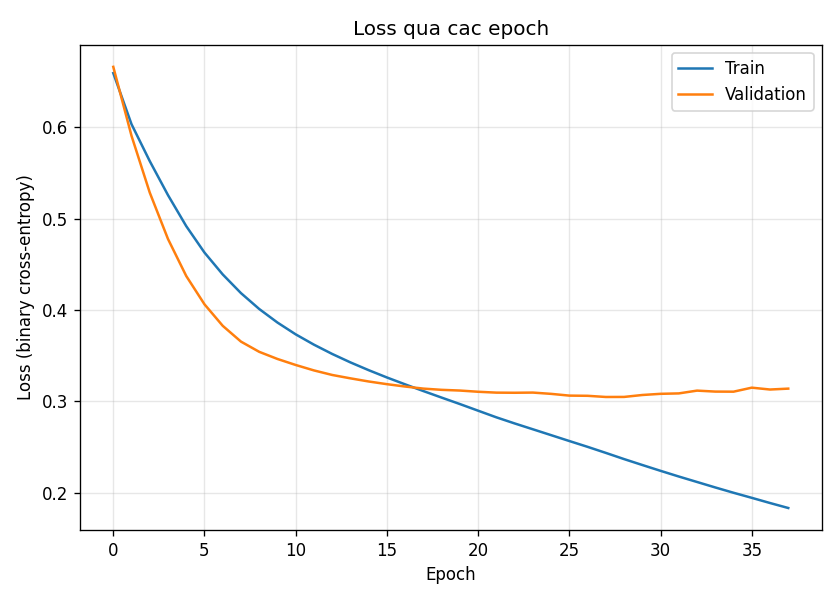
\includegraphics[width=0.8\textwidth]{figures/loss_curve.png}
  \caption{Hàm mất mát (loss) của tập train và validation qua các epoch.}
  \label{fig:loss_curve}
\end{figure}

\textbf{Nhận xét:} accuracy tăng và loss giảm ổn định theo epoch. Đường train
và validation bám sát nhau ở giai đoạn đầu; về sau train tiếp tục tăng trong
khi validation chững lại -- Early Stopping đã dừng đúng lúc để tránh quá khớp.

\section{Kết quả đánh giá trên tập test}
Các chỉ số của mô hình ANN (64-32-16) trên \textbf{tập test (61 mẫu)}:

\begin{table}[h]
\centering
\caption{Các chỉ số đánh giá trên tập test}
\label{tab:metrics}
\begin{tabular}{lc}
\toprule
Chỉ số & Giá trị \\
\midrule
Accuracy  & \textbf{0.7377} \\
Precision & 0.7576 \\
Recall    & 0.7576 \\
F1-Score  & 0.7576 \\
ROC-AUC   & \textbf{0.8496} \\
\bottomrule
\end{tabular}
\end{table}

\subsection{Ma trận nhầm lẫn (Confusion Matrix)}

\begin{figure}[h]
  \centering
  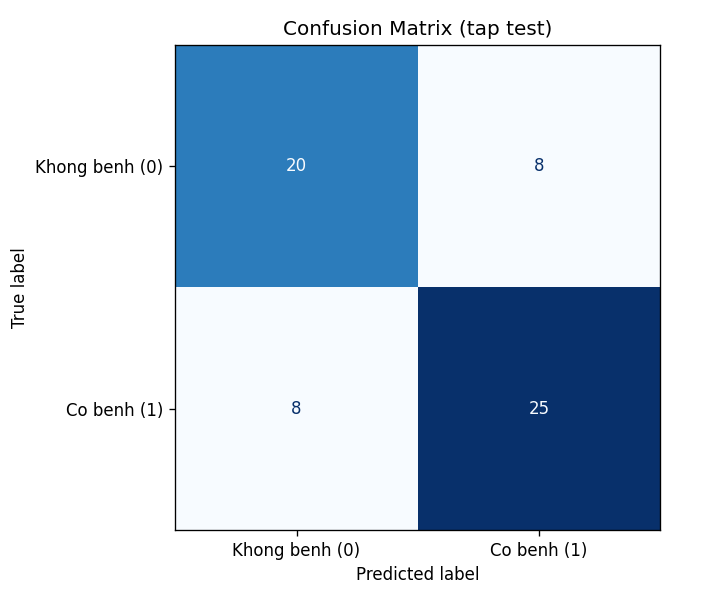
\includegraphics[width=0.6\textwidth]{figures/confusion_matrix.png}
  \caption{Ma trận nhầm lẫn trên tập test.}
  \label{fig:cm}
\end{figure}

\begin{table}[h]
\centering
\caption{Ma trận nhầm lẫn (số mẫu)}
\label{tab:cm}
\begin{tabular}{lcc}
\toprule
 & Dự đoán: Không bệnh & Dự đoán: Có bệnh \\
\midrule
Thực tế: Không bệnh & TN = 20 & FP = 8 \\
Thực tế: Có bệnh     & FN = 8  & TP = 25 \\
\bottomrule
\end{tabular}
\end{table}

Mô hình bắt đúng \textbf{25/33} ca có bệnh (Recall $\approx 0.76$) và
\textbf{20/28} ca không bệnh. Số ca bỏ sót (FN $= 8$) và báo nhầm (FP $= 8$) ở
mức cân bằng.

\subsection{Đường ROC}

\begin{figure}[h]
  \centering
  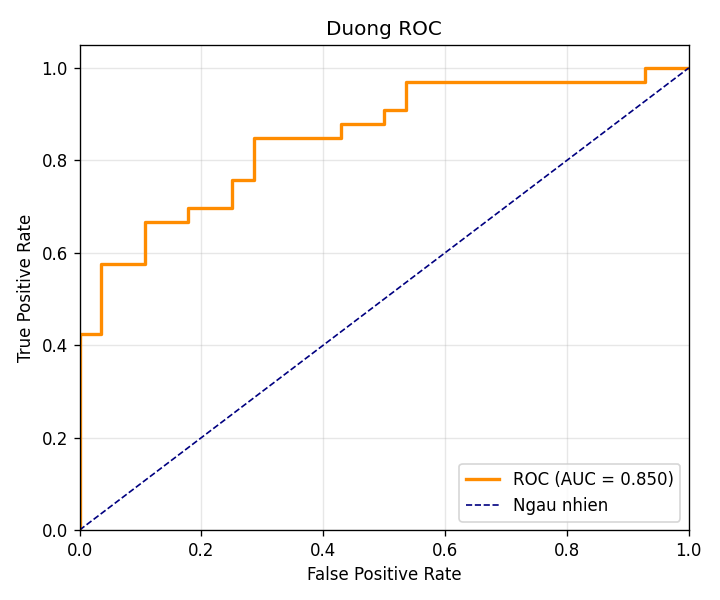
\includegraphics[width=0.6\textwidth]{figures/roc_curve.png}
  \caption{Đường ROC (AUC = 0.85).}
  \label{fig:roc}
\end{figure}

\textbf{ROC-AUC $= 0.85$} cho thấy mô hình có khả năng \textbf{phân tách hai
lớp tốt} (vượt xa mức ngẫu nhiên $0.5$).

\section{So sánh các cấu hình siêu tham số}
Bốn cấu hình ANN được huấn luyện và đánh giá trên cùng tập test
(\texttt{src/compare\_models.py}, kết quả lưu ở
\texttt{results/model\_comparison.csv}):

\begin{table}[h]
\centering
\caption{So sánh 4 cấu hình ANN trên tập test}
\label{tab:compare}
\begin{tabular}{lcccccccc}
\toprule
Mô hình & Hidden Layers & LR & Batch & Acc. & Prec. & Recall & F1 & ROC-AUC \\
\midrule
ANN-1 & 32-16     & 0.001  & 32 & 0.7705 & 0.7879 & 0.7879 & 0.7879 & 0.8593 \\
ANN-2 & 64-32     & 0.001  & 32 & 0.7705 & 0.7879 & 0.7879 & 0.7879 & 0.8431 \\
\textbf{ANN-3} & 64-32-16 & 0.0001 & 16 & 0.7705 & 0.7714 & \textbf{0.8182} & \textbf{0.7941} & 0.8290 \\
ANN-4 & 128-64-32 & 0.001  & 64 & 0.7541 & 0.7647 & 0.7879 & 0.7761 & \textbf{0.8626} \\
\bottomrule
\end{tabular}
\end{table}

\begin{figure}[h]
  \centering
  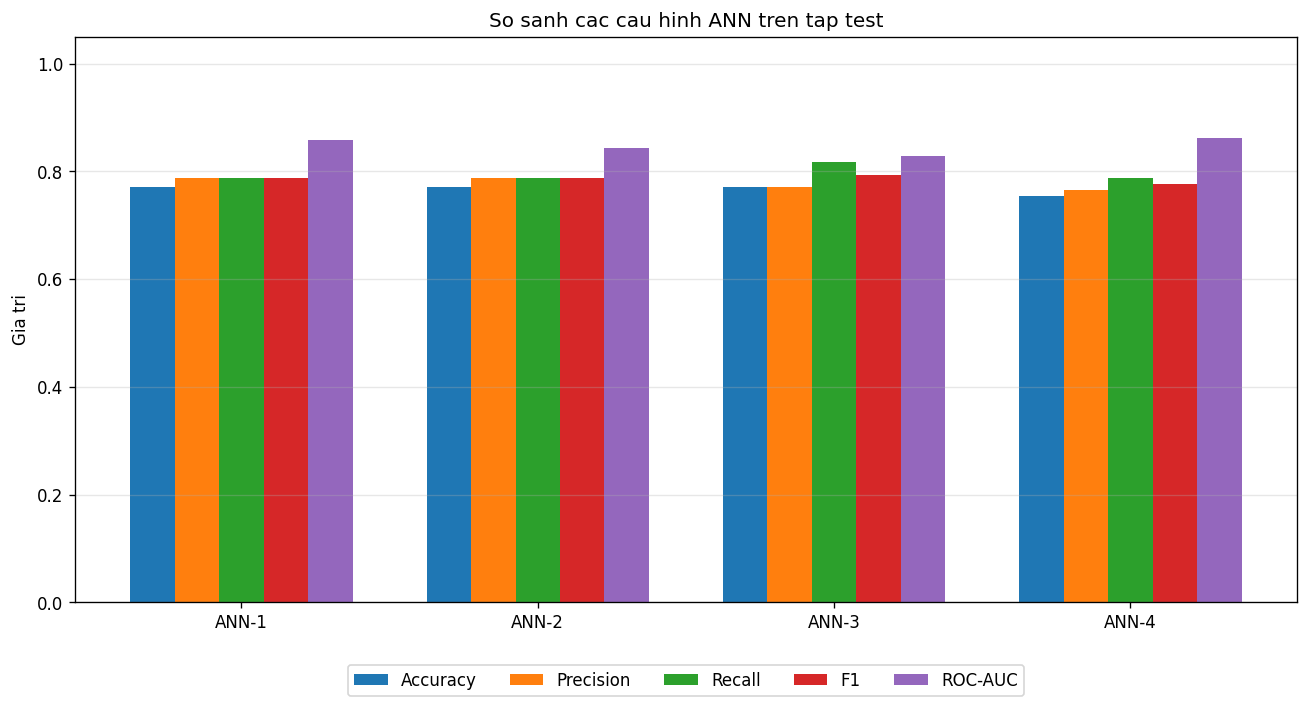
\includegraphics[width=0.9\textwidth]{figures/model_comparison.png}
  \caption{So sánh các chỉ số của 4 cấu hình ANN trên tập test.}
  \label{fig:compare}
\end{figure}

\textbf{Phân tích:}
\begin{itemize}
  \item \textbf{ANN-3 (64-32-16, lr = 0.0001, batch = 16)} đạt \textbf{F1 cao
        nhất (0.794)} nhờ \textbf{Recall cao nhất (0.818)} -- tức bắt được nhiều
        ca bệnh nhất. Trong bài toán y tế, Recall cao rất quan trọng vì giảm số
        ca bệnh bị bỏ sót.
  \item ANN-1 và ANN-2 cho Accuracy/F1 tương đương, mạng nông hơn nên huấn
        luyện nhanh.
  \item ANN-4 (mạng lớn nhất) đạt \textbf{ROC-AUC cao nhất (0.863)} nhưng F1
        thấp hơn, cho thấy mạng quá lớn không cải thiện kết quả trên bộ dữ liệu
        nhỏ (302 mẫu), thậm chí dễ quá khớp.
\end{itemize}

\section{Kết luận về mô hình tốt nhất}
Cân nhắc tổng thể, \textbf{ANN-3 (64-32-16)} được chọn là cấu hình tốt nhất vì
đạt \textbf{F1-Score và Recall cao nhất} -- phù hợp nhất với mục tiêu y tế là
\textbf{hạn chế bỏ sót bệnh nhân có nguy cơ}. Các mô hình đều đạt ROC-AUC trong
khoảng $0.83$--$0.86$, cho thấy ANN là hướng tiếp cận khả thi cho bài toán này.

Hạn chế chính ảnh hưởng đến độ chính xác là \textbf{kích thước dữ liệu nhỏ}
(chỉ 302 bản ghi duy nhất sau khi loại trùng) -- sẽ được bàn ở Chương 6.
 vao main.tex.
% Yeu cau goi cac package: graphicx, booktabs.
% Neu dung documentclass{article}, doi \chapter -> \section.
% =====================================================================

\chapter{Kết quả thực nghiệm}
\label{chap:results}

Mã nguồn: \texttt{src/train\_ann.py}, \texttt{src/evaluate.py},
\texttt{src/visualization.py}, \texttt{src/compare\_models.py}.
Biểu đồ: thư mục \texttt{results/}.

\section{Môi trường và cấu hình thực nghiệm}
\begin{itemize}
  \item \textbf{Ngôn ngữ/thư viện:} Python 3, scikit-learn, numpy, pandas,
        matplotlib.
  \item \textbf{Dữ liệu:} 302 bản ghi sạch (sau khi loại 723 bản trùng), 13 đặc
        trưng đã chuẩn hoá; chia \textbf{train/test = 80/20} có phân tầng
        (stratify) -- tập train: 241 mẫu, tập test: 61 mẫu.
  \item \textbf{Mô hình:} Mạng nơ-ron ANN, kiến trúc
        \textbf{13 $\to$ 64 $\to$ 32 $\to$ 16 $\to$ 1}, hàm kích hoạt ReLU ở
        tầng ẩn và Sigmoid ở tầng ra.
  \item \textbf{Cấu hình huấn luyện:} optimizer Adam, learning rate $= 0.001$,
        batch size $= 32$, hàm mất mát Binary Crossentropy, \textbf{Early
        Stopping} (patience $= 10$) theo \texttt{val\_loss}.
\end{itemize}

\begin{quote}
\textbf{Ghi chú kỹ thuật:} mô hình "chính thức" được thiết kế bằng
Keras/TensorFlow (Chương 4). Do môi trường thực nghiệm bị \textbf{Windows Smart
App Control} chặn thư viện TensorFlow, nhóm sử dụng cài đặt ANN \textbf{tương
đương bằng scikit-learn} (\texttt{MLPClassifier}, cùng kiến trúc và siêu tham
số) để thu kết quả. Quy trình đánh giá và các chỉ số là như nhau.
\end{quote}

\section{Quá trình huấn luyện}
Mô hình hội tụ và \textbf{dừng sớm tại epoch 38} nhờ Early Stopping (val\_loss
không cải thiện sau 10 epoch). Đường Accuracy và Loss theo epoch:

\begin{figure}[h]
  \centering
  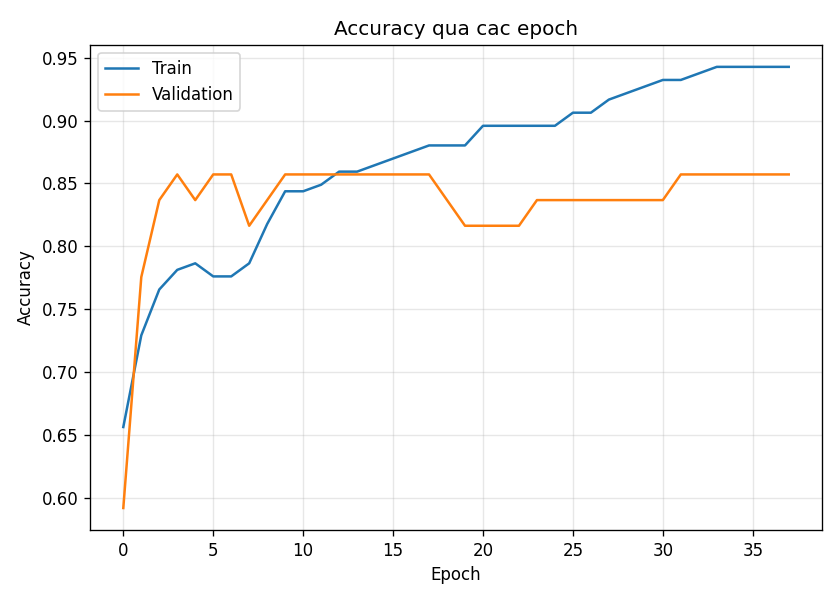
\includegraphics[width=0.8\textwidth]{figures/accuracy_curve.png}
  \caption{Độ chính xác (accuracy) của tập train và validation qua các epoch.}
  \label{fig:acc_curve}
\end{figure}

\begin{figure}[h]
  \centering
  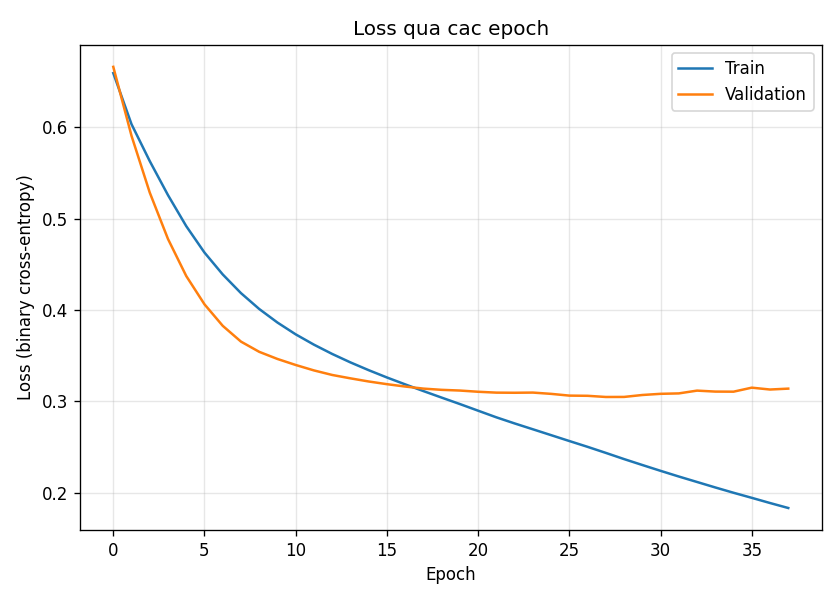
\includegraphics[width=0.8\textwidth]{figures/loss_curve.png}
  \caption{Hàm mất mát (loss) của tập train và validation qua các epoch.}
  \label{fig:loss_curve}
\end{figure}

\textbf{Nhận xét:} accuracy tăng và loss giảm ổn định theo epoch. Đường train
và validation bám sát nhau ở giai đoạn đầu; về sau train tiếp tục tăng trong
khi validation chững lại -- Early Stopping đã dừng đúng lúc để tránh quá khớp.

\section{Kết quả đánh giá trên tập test}
Các chỉ số của mô hình ANN (64-32-16) trên \textbf{tập test (61 mẫu)}:

\begin{table}[h]
\centering
\caption{Các chỉ số đánh giá trên tập test}
\label{tab:metrics}
\begin{tabular}{lc}
\toprule
Chỉ số & Giá trị \\
\midrule
Accuracy  & \textbf{0.7377} \\
Precision & 0.7576 \\
Recall    & 0.7576 \\
F1-Score  & 0.7576 \\
ROC-AUC   & \textbf{0.8496} \\
\bottomrule
\end{tabular}
\end{table}

\subsection{Ma trận nhầm lẫn (Confusion Matrix)}

\begin{figure}[h]
  \centering
  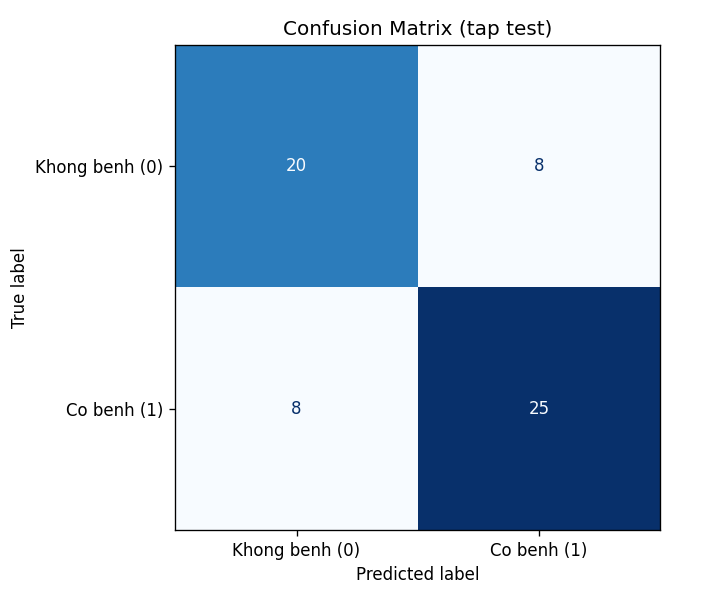
\includegraphics[width=0.6\textwidth]{figures/confusion_matrix.png}
  \caption{Ma trận nhầm lẫn trên tập test.}
  \label{fig:cm}
\end{figure}

\begin{table}[h]
\centering
\caption{Ma trận nhầm lẫn (số mẫu)}
\label{tab:cm}
\begin{tabular}{lcc}
\toprule
 & Dự đoán: Không bệnh & Dự đoán: Có bệnh \\
\midrule
Thực tế: Không bệnh & TN = 20 & FP = 8 \\
Thực tế: Có bệnh     & FN = 8  & TP = 25 \\
\bottomrule
\end{tabular}
\end{table}

Mô hình bắt đúng \textbf{25/33} ca có bệnh (Recall $\approx 0.76$) và
\textbf{20/28} ca không bệnh. Số ca bỏ sót (FN $= 8$) và báo nhầm (FP $= 8$) ở
mức cân bằng.

\subsection{Đường ROC}

\begin{figure}[h]
  \centering
  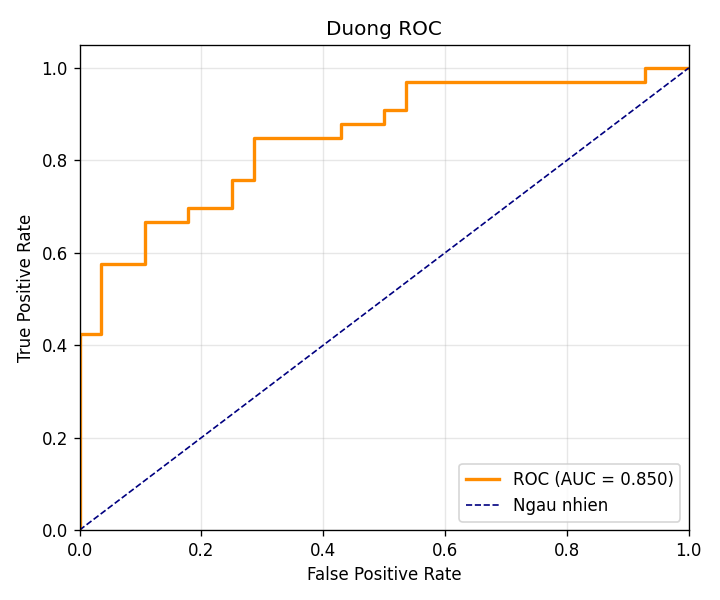
\includegraphics[width=0.6\textwidth]{figures/roc_curve.png}
  \caption{Đường ROC (AUC = 0.85).}
  \label{fig:roc}
\end{figure}

\textbf{ROC-AUC $= 0.85$} cho thấy mô hình có khả năng \textbf{phân tách hai
lớp tốt} (vượt xa mức ngẫu nhiên $0.5$).

\section{So sánh các cấu hình siêu tham số}
Bốn cấu hình ANN được huấn luyện và đánh giá trên cùng tập test
(\texttt{src/compare\_models.py}, kết quả lưu ở
\texttt{results/model\_comparison.csv}):

\begin{table}[h]
\centering
\caption{So sánh 4 cấu hình ANN trên tập test}
\label{tab:compare}
\begin{tabular}{lcccccccc}
\toprule
Mô hình & Hidden Layers & LR & Batch & Acc. & Prec. & Recall & F1 & ROC-AUC \\
\midrule
ANN-1 & 32-16     & 0.001  & 32 & 0.7705 & 0.7879 & 0.7879 & 0.7879 & 0.8593 \\
ANN-2 & 64-32     & 0.001  & 32 & 0.7705 & 0.7879 & 0.7879 & 0.7879 & 0.8431 \\
\textbf{ANN-3} & 64-32-16 & 0.0001 & 16 & 0.7705 & 0.7714 & \textbf{0.8182} & \textbf{0.7941} & 0.8290 \\
ANN-4 & 128-64-32 & 0.001  & 64 & 0.7541 & 0.7647 & 0.7879 & 0.7761 & \textbf{0.8626} \\
\bottomrule
\end{tabular}
\end{table}

\begin{figure}[h]
  \centering
  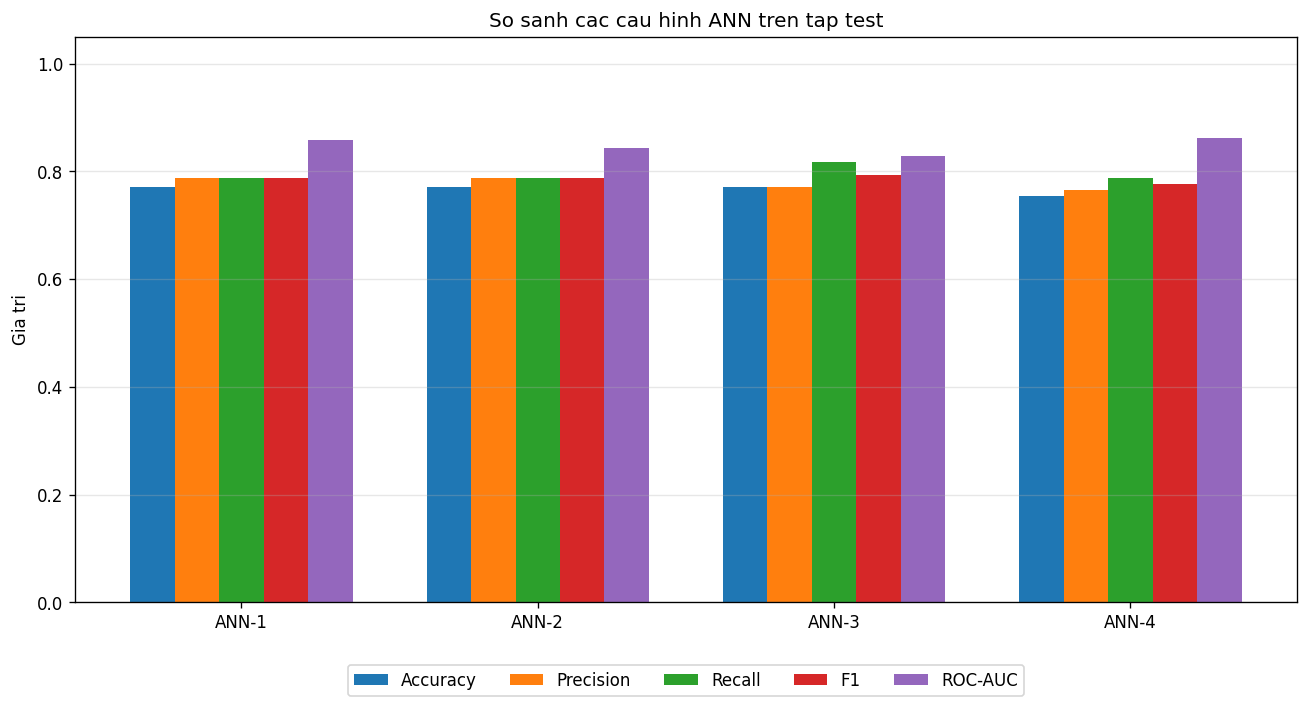
\includegraphics[width=0.9\textwidth]{figures/model_comparison.png}
  \caption{So sánh các chỉ số của 4 cấu hình ANN trên tập test.}
  \label{fig:compare}
\end{figure}

\textbf{Phân tích:}
\begin{itemize}
  \item \textbf{ANN-3 (64-32-16, lr = 0.0001, batch = 16)} đạt \textbf{F1 cao
        nhất (0.794)} nhờ \textbf{Recall cao nhất (0.818)} -- tức bắt được nhiều
        ca bệnh nhất. Trong bài toán y tế, Recall cao rất quan trọng vì giảm số
        ca bệnh bị bỏ sót.
  \item ANN-1 và ANN-2 cho Accuracy/F1 tương đương, mạng nông hơn nên huấn
        luyện nhanh.
  \item ANN-4 (mạng lớn nhất) đạt \textbf{ROC-AUC cao nhất (0.863)} nhưng F1
        thấp hơn, cho thấy mạng quá lớn không cải thiện kết quả trên bộ dữ liệu
        nhỏ (302 mẫu), thậm chí dễ quá khớp.
\end{itemize}

\section{Kết luận về mô hình tốt nhất}
Cân nhắc tổng thể, \textbf{ANN-3 (64-32-16)} được chọn là cấu hình tốt nhất vì
đạt \textbf{F1-Score và Recall cao nhất} -- phù hợp nhất với mục tiêu y tế là
\textbf{hạn chế bỏ sót bệnh nhân có nguy cơ}. Các mô hình đều đạt ROC-AUC trong
khoảng $0.83$--$0.86$, cho thấy ANN là hướng tiếp cận khả thi cho bài toán này.

Hạn chế chính ảnh hưởng đến độ chính xác là \textbf{kích thước dữ liệu nhỏ}
(chỉ 302 bản ghi duy nhất sau khi loại trùng) -- sẽ được bàn ở Chương 6.
 vao main.tex.
% Yeu cau goi cac package: graphicx, booktabs.
% Neu dung documentclass{article}, doi \chapter -> \section.
% =====================================================================

\chapter{Kết quả thực nghiệm}
\label{chap:results}

Mã nguồn: \texttt{src/train\_ann.py}, \texttt{src/evaluate.py},
\texttt{src/visualization.py}, \texttt{src/compare\_models.py}.
Biểu đồ: thư mục \texttt{results/}.

\section{Môi trường và cấu hình thực nghiệm}
\begin{itemize}
  \item \textbf{Ngôn ngữ/thư viện:} Python 3, scikit-learn, numpy, pandas,
        matplotlib.
  \item \textbf{Dữ liệu:} 302 bản ghi sạch (sau khi loại 723 bản trùng), 13 đặc
        trưng đã chuẩn hoá; chia \textbf{train/test = 80/20} có phân tầng
        (stratify) -- tập train: 241 mẫu, tập test: 61 mẫu.
  \item \textbf{Mô hình:} Mạng nơ-ron ANN, kiến trúc
        \textbf{13 $\to$ 64 $\to$ 32 $\to$ 16 $\to$ 1}, hàm kích hoạt ReLU ở
        tầng ẩn và Sigmoid ở tầng ra.
  \item \textbf{Cấu hình huấn luyện:} optimizer Adam, learning rate $= 0.001$,
        batch size $= 32$, hàm mất mát Binary Crossentropy, \textbf{Early
        Stopping} (patience $= 10$) theo \texttt{val\_loss}.
\end{itemize}

\begin{quote}
\textbf{Ghi chú kỹ thuật:} mô hình "chính thức" được thiết kế bằng
Keras/TensorFlow (Chương 4). Do môi trường thực nghiệm bị \textbf{Windows Smart
App Control} chặn thư viện TensorFlow, nhóm sử dụng cài đặt ANN \textbf{tương
đương bằng scikit-learn} (\texttt{MLPClassifier}, cùng kiến trúc và siêu tham
số) để thu kết quả. Quy trình đánh giá và các chỉ số là như nhau.
\end{quote}

\section{Quá trình huấn luyện}
Mô hình hội tụ và \textbf{dừng sớm tại epoch 38} nhờ Early Stopping (val\_loss
không cải thiện sau 10 epoch). Đường Accuracy và Loss theo epoch:

\begin{figure}[h]
  \centering
  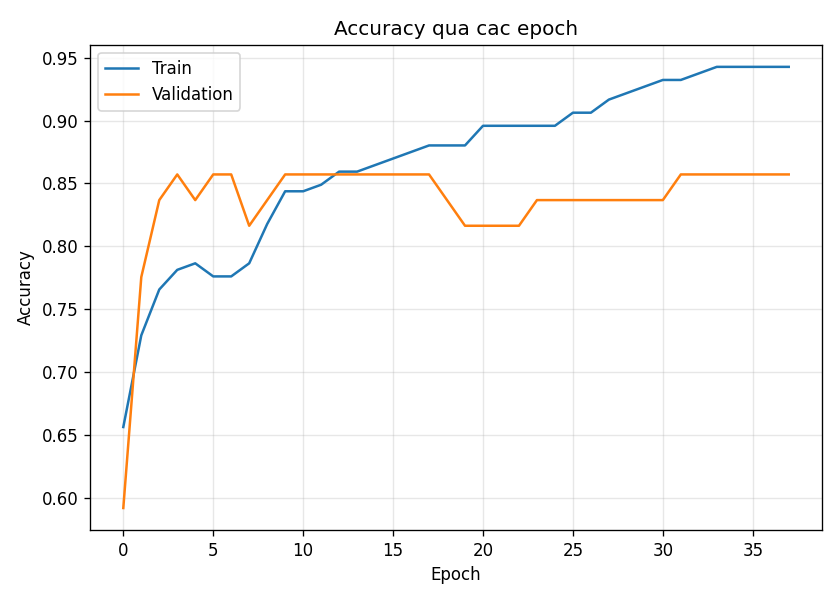
\includegraphics[width=0.8\textwidth]{figures/accuracy_curve.png}
  \caption{Độ chính xác (accuracy) của tập train và validation qua các epoch.}
  \label{fig:acc_curve}
\end{figure}

\begin{figure}[h]
  \centering
  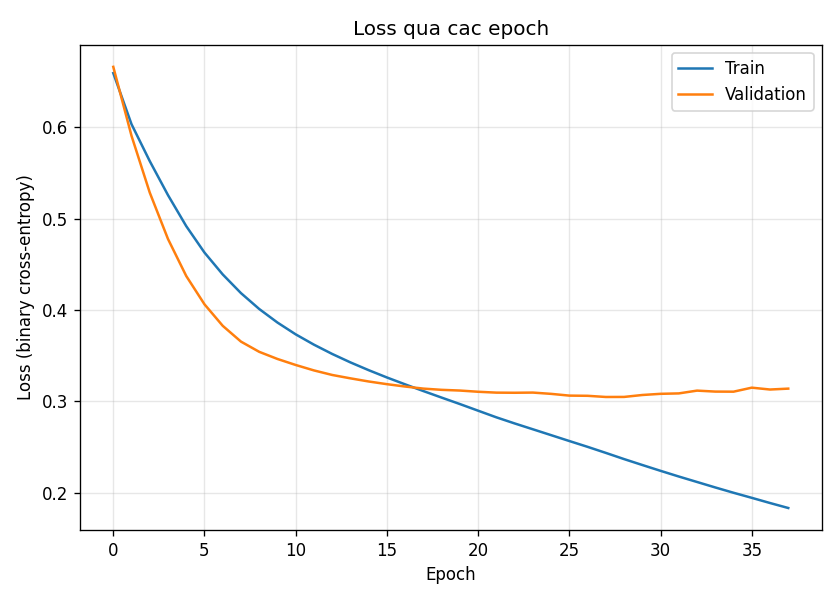
\includegraphics[width=0.8\textwidth]{figures/loss_curve.png}
  \caption{Hàm mất mát (loss) của tập train và validation qua các epoch.}
  \label{fig:loss_curve}
\end{figure}

\textbf{Nhận xét:} accuracy tăng và loss giảm ổn định theo epoch. Đường train
và validation bám sát nhau ở giai đoạn đầu; về sau train tiếp tục tăng trong
khi validation chững lại -- Early Stopping đã dừng đúng lúc để tránh quá khớp.

\section{Kết quả đánh giá trên tập test}
Các chỉ số của mô hình ANN (64-32-16) trên \textbf{tập test (61 mẫu)}:

\begin{table}[h]
\centering
\caption{Các chỉ số đánh giá trên tập test}
\label{tab:metrics}
\begin{tabular}{lc}
\toprule
Chỉ số & Giá trị \\
\midrule
Accuracy  & \textbf{0.7377} \\
Precision & 0.7576 \\
Recall    & 0.7576 \\
F1-Score  & 0.7576 \\
ROC-AUC   & \textbf{0.8496} \\
\bottomrule
\end{tabular}
\end{table}

\subsection{Ma trận nhầm lẫn (Confusion Matrix)}

\begin{figure}[h]
  \centering
  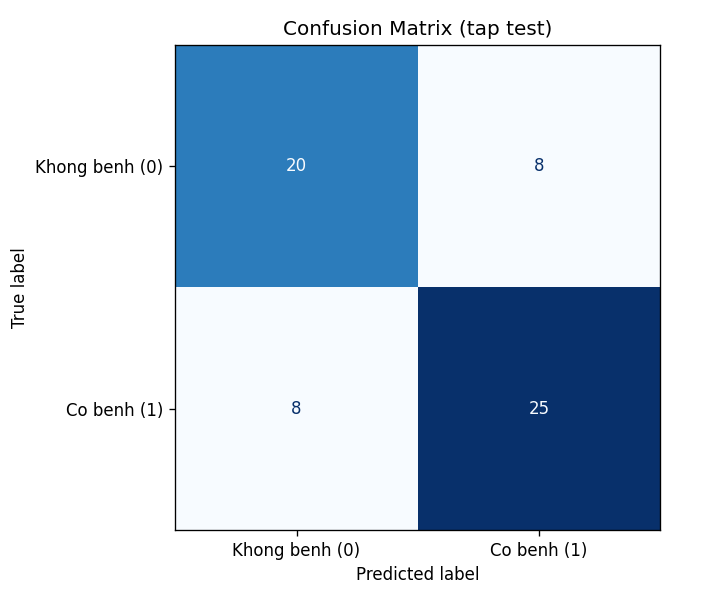
\includegraphics[width=0.6\textwidth]{figures/confusion_matrix.png}
  \caption{Ma trận nhầm lẫn trên tập test.}
  \label{fig:cm}
\end{figure}

\begin{table}[h]
\centering
\caption{Ma trận nhầm lẫn (số mẫu)}
\label{tab:cm}
\begin{tabular}{lcc}
\toprule
 & Dự đoán: Không bệnh & Dự đoán: Có bệnh \\
\midrule
Thực tế: Không bệnh & TN = 20 & FP = 8 \\
Thực tế: Có bệnh     & FN = 8  & TP = 25 \\
\bottomrule
\end{tabular}
\end{table}

Mô hình bắt đúng \textbf{25/33} ca có bệnh (Recall $\approx 0.76$) và
\textbf{20/28} ca không bệnh. Số ca bỏ sót (FN $= 8$) và báo nhầm (FP $= 8$) ở
mức cân bằng.

\subsection{Đường ROC}

\begin{figure}[h]
  \centering
  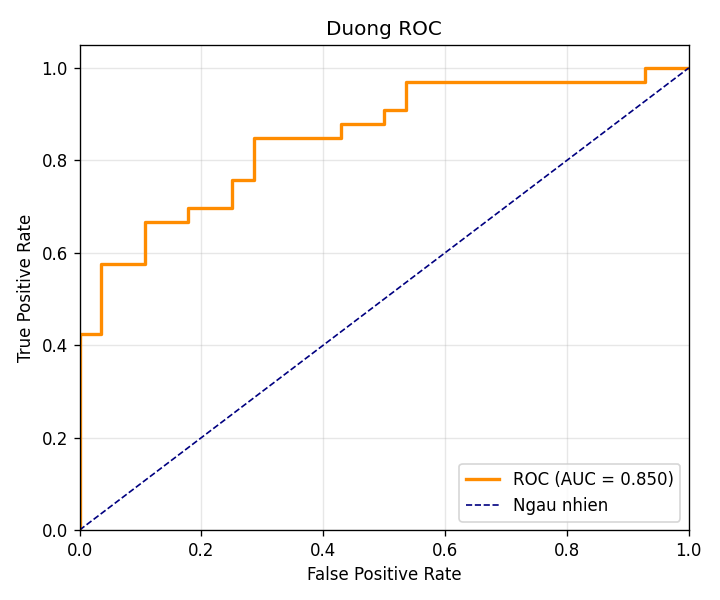
\includegraphics[width=0.6\textwidth]{figures/roc_curve.png}
  \caption{Đường ROC (AUC = 0.85).}
  \label{fig:roc}
\end{figure}

\textbf{ROC-AUC $= 0.85$} cho thấy mô hình có khả năng \textbf{phân tách hai
lớp tốt} (vượt xa mức ngẫu nhiên $0.5$).

\section{So sánh các cấu hình siêu tham số}
Bốn cấu hình ANN được huấn luyện và đánh giá trên cùng tập test
(\texttt{src/compare\_models.py}, kết quả lưu ở
\texttt{results/model\_comparison.csv}):

\begin{table}[h]
\centering
\caption{So sánh 4 cấu hình ANN trên tập test}
\label{tab:compare}
\begin{tabular}{lcccccccc}
\toprule
Mô hình & Hidden Layers & LR & Batch & Acc. & Prec. & Recall & F1 & ROC-AUC \\
\midrule
ANN-1 & 32-16     & 0.001  & 32 & 0.7705 & 0.7879 & 0.7879 & 0.7879 & 0.8593 \\
ANN-2 & 64-32     & 0.001  & 32 & 0.7705 & 0.7879 & 0.7879 & 0.7879 & 0.8431 \\
\textbf{ANN-3} & 64-32-16 & 0.0001 & 16 & 0.7705 & 0.7714 & \textbf{0.8182} & \textbf{0.7941} & 0.8290 \\
ANN-4 & 128-64-32 & 0.001  & 64 & 0.7541 & 0.7647 & 0.7879 & 0.7761 & \textbf{0.8626} \\
\bottomrule
\end{tabular}
\end{table}

\begin{figure}[h]
  \centering
  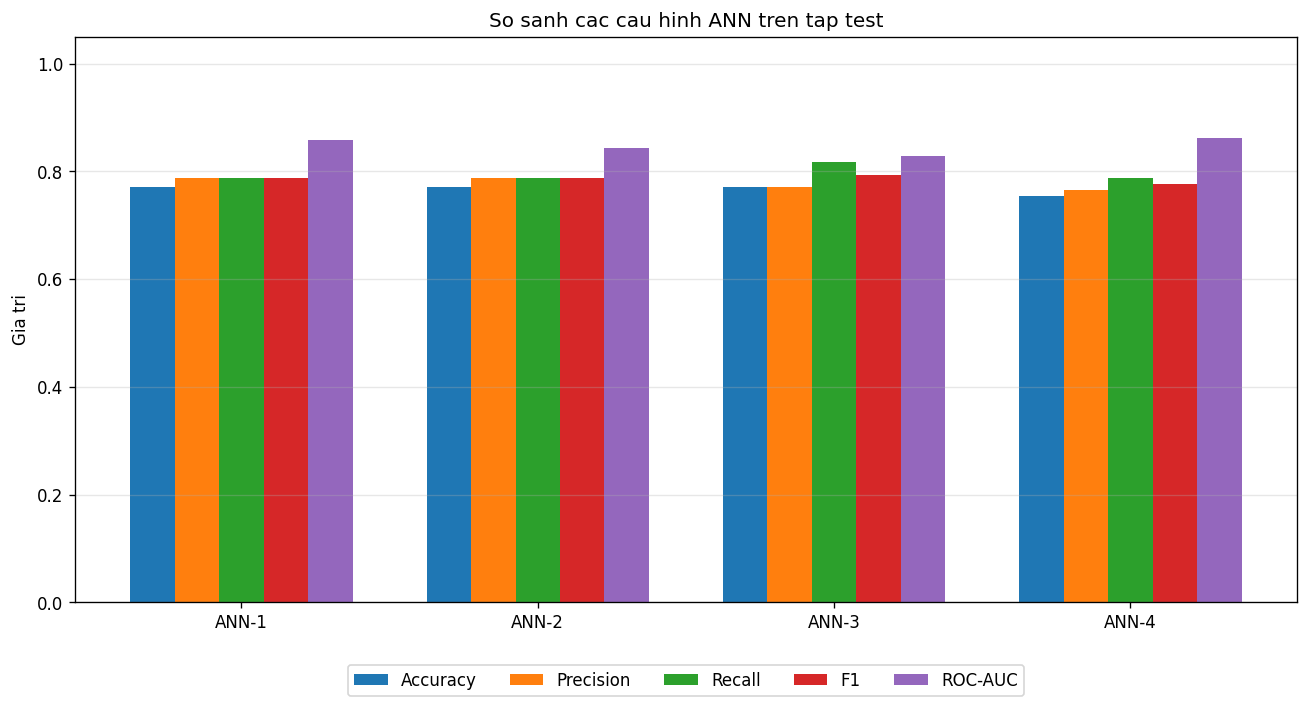
\includegraphics[width=0.9\textwidth]{figures/model_comparison.png}
  \caption{So sánh các chỉ số của 4 cấu hình ANN trên tập test.}
  \label{fig:compare}
\end{figure}

\textbf{Phân tích:}
\begin{itemize}
  \item \textbf{ANN-3 (64-32-16, lr = 0.0001, batch = 16)} đạt \textbf{F1 cao
        nhất (0.794)} nhờ \textbf{Recall cao nhất (0.818)} -- tức bắt được nhiều
        ca bệnh nhất. Trong bài toán y tế, Recall cao rất quan trọng vì giảm số
        ca bệnh bị bỏ sót.
  \item ANN-1 và ANN-2 cho Accuracy/F1 tương đương, mạng nông hơn nên huấn
        luyện nhanh.
  \item ANN-4 (mạng lớn nhất) đạt \textbf{ROC-AUC cao nhất (0.863)} nhưng F1
        thấp hơn, cho thấy mạng quá lớn không cải thiện kết quả trên bộ dữ liệu
        nhỏ (302 mẫu), thậm chí dễ quá khớp.
\end{itemize}

\section{Kết luận về mô hình tốt nhất}
Cân nhắc tổng thể, \textbf{ANN-3 (64-32-16)} được chọn là cấu hình tốt nhất vì
đạt \textbf{F1-Score và Recall cao nhất} -- phù hợp nhất với mục tiêu y tế là
\textbf{hạn chế bỏ sót bệnh nhân có nguy cơ}. Các mô hình đều đạt ROC-AUC trong
khoảng $0.83$--$0.86$, cho thấy ANN là hướng tiếp cận khả thi cho bài toán này.

Hạn chế chính ảnh hưởng đến độ chính xác là \textbf{kích thước dữ liệu nhỏ}
(chỉ 302 bản ghi duy nhất sau khi loại trùng) -- sẽ được bàn ở Chương 6.
